\documentclass[9pt,aspectratio=169]{beamer}

% ============================================================
% PACKAGES
% ============================================================
\usepackage[utf8]{inputenc}
\usepackage[T1]{fontenc}
\usepackage{amsmath,amssymb}
\usepackage{graphicx}
\usepackage[table]{xcolor}
\usepackage{booktabs}
\usepackage{multirow}
\usepackage{array}
\usepackage{hyperref}
\usepackage{lmodern}
\usepackage{tikz}
\usetikzlibrary{positioning,arrows.meta,calc,shapes.multipart}

% ============================================================
% THEME
% ============================================================
\usetheme{Madrid}
\usecolortheme{seahorse}
\setbeamertemplate{navigation symbols}{}
\setbeamertemplate{footline}{%
  \leavevmode%
  \hbox{%
    \begin{beamercolorbox}[wd=.5\paperwidth,ht=2.25ex,dp=1ex,left,leftskip=1em]{author in head/foot}%
      \usebeamerfont{author in head/foot}\insertshortauthor\ |\ \insertshortinstitute
    \end{beamercolorbox}%
    \begin{beamercolorbox}[wd=.4\paperwidth,ht=2.25ex,dp=1ex,center]{title in head/foot}%
      \usebeamerfont{title in head/foot}\insertshorttitle
    \end{beamercolorbox}%
    \begin{beamercolorbox}[wd=.1\paperwidth,ht=2.25ex,dp=1ex,right,rightskip=1em]{date in head/foot}%
      \usebeamerfont{date in head/foot}\insertframenumber/\inserttotalframenumber
    \end{beamercolorbox}}%
}
\setbeamerfont{frametitle}{size=\small,series=\bfseries}
\setbeamerfont{title}{size=\large,series=\bfseries}
\setbeamerfont{subtitle}{size=\footnotesize}
\setbeamerfont{block title}{size=\footnotesize,series=\bfseries}
\setbeamerfont{block body}{size=\footnotesize}
\setbeamertemplate{itemize items}[circle]
\setbeamertemplate{enumerate items}[default]

\setlength{\leftmargini}{1.1em}
\setlength{\leftmarginii}{0.9em}
\setlength{\itemsep}{0pt}
\setlength{\parskip}{0pt}

% ============================================================
% COLOURS
% ============================================================
\definecolor{darkred}{RGB}{150,20,20}
\definecolor{steelblue}{RGB}{50,90,160}
\definecolor{forestgreen}{RGB}{30,110,50}
\definecolor{amberc}{RGB}{200,140,20}

% ============================================================
% TITLE PAGE
% ============================================================
\title[Banking Credit Risk Platform]{%
  Banking Credit Risk Calculator}

\subtitle{Solution Walkthrough}

\author[Credit Risk Engineering]{Credit Risk \& Banking Intelligence Platform}

\institute[Axis Bank]{%
  Banking Credit Risk Calculator --- Internal Solution Overview}

\date{July 2026}

% ============================================================
\begin{document}
% ============================================================

% SLIDE — TITLE
\begin{frame}
  \titlepage
\end{frame}

% SLIDE — OUTLINE
\begin{frame}{Outline}
  \tableofcontents
\end{frame}

% ===========================================================
\section{The Data}
% ===========================================================

% SLIDE — BANK PORTFOLIO SUMMARY
\begin{frame}{Our Banks --- Portfolio Summary (FY2026)}
\vspace{-2pt}
{\footnotesize Nine banks, grounded in a real per-loan ledger --- every figure below is
computed directly from \texttt{bank.db} (balance sheet + loan book), not estimated.}\\[6pt]
\begin{center}
\scriptsize
\setlength{\tabcolsep}{3.5pt}
\begin{tabular}{lp{2.1cm}rrrrrr}
  \toprule
  \textbf{Bank} & \textbf{Country} & \textbf{Total Assets (Rs.\,Cr)} & \textbf{Total Liabilities (Rs.\,Cr)} & \textbf{Loans \& Advances (Rs.\,Cr)} & \textbf{Customers} & \textbf{Loans} & \textbf{Defaults}\\
  \midrule
  HDFC Bank             & India           & 191.3 & 191.3 & 130.5 & 2{,}213 & 2{,}045 & 215\\
  ICICI Bank             & India           & 202.3 & 202.3 & 138.0 & 2{,}275 & 2{,}132 & 228\\
  JPMorgan Chase N.A.    & United States   & 173.6 & 173.6 & 118.4 & 2{,}277 & 2{,}112 & 215\\
  Barclays Bank PLC      & United Kingdom  & 150.7 & 150.7 & 102.8 & 2{,}419 & 2{,}215 & 216\\
  DBS Bank Ltd           & Singapore       & 201.9 & 201.9 & 137.7 & 2{,}341 & 2{,}169 & 211\\
  Emirates NBD           & UAE             & 190.4 & 190.4 & 129.8 & 2{,}339 & 2{,}169 & 216\\
  Bank of Baroda          & India           & 212.5 & 212.5 & 144.9 & 2{,}108 & 1{,}961 & 223\\
  Commonwealth Bank       & Australia       & 184.8 & 184.8 & 126.0 & 2{,}203 & 2{,}035 & 212\\
  Punjab National Bank   & India           & 206.8 & 206.8 & 141.0 & 2{,}448 & 2{,}317 & 216\\
  \midrule
  \textbf{Total (9 banks)} & --- & \textbf{1{,}714.5} & \textbf{1{,}714.5} & \textbf{1{,}169.2} & \textbf{20{,}623} & \textbf{19{,}155} & \textbf{1{,}952}\\
  \bottomrule
\end{tabular}
\end{center}
\vspace{6pt}
\begin{alertblock}{How these numbers are derived}
  \footnotesize
  Total Assets/Liabilities from \texttt{bank\_balance\_sheet} (FY2026, as-on 2026-03-31) --- the two
  always tie out exactly, as required by double-entry accounting. Loans \& Advances is the
  \texttt{advances\_net} balance-sheet line (the active loan book). Customers and Loans are row
  counts from \texttt{customers} and \texttt{loans}. Defaults = loans classified
  \texttt{Written-Off} --- the platform's realised-default definition.
\end{alertblock}
\end{frame}

% SLIDE — EXPOSURE TYPES
\begin{frame}{Exposure Types --- Customers \& Defaults (All 9 Banks, Aggregated)}
\vspace{-2pt}
{\footnotesize The platform scores every borrower under one of four Basel exposure classes ---
each routed to its own PD model. Figures below are aggregated across all 9 banks.}\\[6pt]
\begin{center}
\footnotesize
\setlength{\tabcolsep}{8pt}
\begin{tabular}{lrrrr}
  \toprule
  \textbf{Exposure Type} & \textbf{Customers} & \textbf{Loans} & \textbf{Defaults} & \textbf{Default Rate}\\
  \midrule
  CORPORATE          &  5{,}070 &  5{,}070 &   488 &  9.63\%\\
  SME                &  4{,}655 &  4{,}655 &   488 & 10.48\%\\
  RETAIL\_MORTGAGES  &  4{,}950 &  4{,}950 &   488 &  9.86\%\\
  RETAIL\_OTHER      &  4{,}479 &  4{,}480 &   488 & 10.89\%\\
  \midrule
  \textbf{Total}     & \textbf{19{,}154} & \textbf{19{,}155} & \textbf{1{,}952} & \textbf{10.19\%}\\
  \bottomrule
\end{tabular}
\end{center}
\vspace{6pt}
\begin{alertblock}{How these numbers are derived}
  \footnotesize
  Customers = distinct borrowers holding at least one loan in that exposure class (\texttt{loans.exposure\_class}).
  Loans = row count in \texttt{loans} for that class. Defaults = loans classified \texttt{Written-Off}
  --- the same realised-default definition used on the previous slide.
\end{alertblock}
\end{frame}

% SLIDE — MODEL FEATURES BY FIVE C
\begin{frame}{Model Training Attributes --- Grouped by the Five C's}
\vspace{-3pt}
{\scriptsize All 4 segment PD models (CORPORATE, SME, RETAIL\_MORTGAGES, RETAIL\_OTHER) are trained
on the same 36-attribute schema (\texttt{ml\_models/pd\_model\_metadata\_*.json}).}\\[3pt]
\begin{columns}[T]
  \column{0.49\textwidth}
    \tiny
    \setlength{\tabcolsep}{2.5pt}
    \renewcommand{\arraystretch}{1.05}
    \begin{tabular}{@{}lp{1.9cm}p{3.1cm}@{}}
      \toprule
      \textbf{5C} & \textbf{Feature} & \textbf{Description}\\
      \midrule
      \multirow{8}{*}{\cellcolor{steelblue!25}\rotatebox{90}{Character}}
        & \texttt{age}                      & Borrower's age (years)\\
        & \texttt{employment\_type\_enc}     & Employment type (encoded)\\
        & \texttt{years\_employed}           & Years in current job\\
        & \texttt{city\_tier\_enc}           & City tier (encoded)\\
        & \texttt{education\_enc}            & Education level (encoded)\\
        & \texttt{cibil\_score}              & Credit bureau score (300--900)\\
        & \texttt{months\_as\_customer}      & Relationship tenure with bank\\
        & \texttt{num\_late\_payments\_\allowbreak past\_12m} & Late payments, past 12 months\\
      \midrule
      \multirow{7}{*}{\cellcolor{orange!25}\rotatebox{90}{Capacity}}
        & \texttt{de\_ratio}                 & Debt-to-equity ratio\\
        & \texttt{interest\_coverage}        & Interest coverage ratio\\
        & \texttt{annual\_income}            & Declared annual income\\
        & \texttt{foir}                      & Fixed obligation-to-income ratio\\
        & \texttt{num\_dependents}           & Number of dependents\\
        & \texttt{loan\_purpose\_enc}        & Loan purpose (encoded)\\
        & \texttt{existing\_loans\_count}    & Count of existing loans\\
      \midrule
      \multirow{4}{*}{\cellcolor{forestgreen!25}\rotatebox{90}{Capital}}
        & \texttt{profitability}             & Net profit margin (\%)\\
        & \texttt{liquidity\_ratio}          & Current ratio (liquidity)\\
        & \texttt{residence\_type\_enc}      & Residence type (owned/rented)\\
        & \texttt{num\_existing\_products}   & Existing product holdings\\
      \midrule
      \cellcolor{darkred!20}Collat.\ & \texttt{ltv\_trend\_pct} & LTV trend since origination (\%)\\
      \bottomrule
    \end{tabular}

  \column{0.49\textwidth}
    \tiny
    \setlength{\tabcolsep}{2.5pt}
    \renewcommand{\arraystretch}{1.05}
    \begin{tabular}{@{}lp{2.1cm}p{2.9cm}@{}}
      \toprule
      \textbf{5C} & \textbf{Feature} & \textbf{Description}\\
      \midrule
      \multirow{16}{*}{\cellcolor{amberc!25}\rotatebox{90}{Conditions}}
        & \texttt{gdp\_growth\_pct}          & GDP growth rate (\%)\\
        & \texttt{inflation\_cpi\_pct}       & CPI inflation rate (\%)\\
        & \texttt{policy\_rate\_pct}         & Central bank policy rate (\%)\\
        & \texttt{unemployment\_pct}         & Unemployment rate (\%)\\
        & \texttt{delta\_de\_ratio}          & Change in leverage since origination\\
        & \texttt{delta\_cibil}              & Change in credit score\\
        & \texttt{months\_since\_\allowbreak origination} & Loan seasoning (months)\\
        & \texttt{delta\_gdp\_pct}           & YoY change in GDP growth\\
        & \texttt{delta\_cpi\_pct}           & YoY change in inflation\\
        & \texttt{delta\_policy\_rate\_pct}  & YoY change in policy rate\\
        & \texttt{delta\_unemployment\_pct}  & YoY change in unemployment\\
        & \texttt{macro\_regime\_score}      & Composite macro distress score (0--100)\\
        & \texttt{ecs\_bounce\_count}        & EMI/ECS bounce count\\
        & \texttt{other\_lender\_emi\_ratio} & EMI ratio owed to other lenders\\
        & \texttt{income\_disruption\_flag}  & Income disruption flag (0/1)\\
        & \texttt{sector\_stress\_index}     & Sector-level stress index\\
      \bottomrule
    \end{tabular}
    \vspace{6pt}

    \begin{block}{\scriptsize Why Conditions dominates}
      \tiny
      Macro, trend, and behavioural-bureau signals change every observation period ---
      they carry most of the schema's breadth even though Character/Capacity drive
      more of the model's actual feature importance.
    \end{block}
\end{columns}
\end{frame}

% SLIDE — WHY XGBOOST & DEPLOYMENT PLAN
\begin{frame}{Why XGBoost, and How We Deploy It}
\vspace{-3pt}
\begin{columns}[T]
  \column{0.52\textwidth}
    \footnotesize\textbf{Why XGBoost (not a simpler model)}
    \begin{itemize}\setlength\itemsep{2pt}\footnotesize
      \item[\small$\bullet$] Handles nonlinear interactions across mixed feature types
            (ratios, encoded categoricals, macro indicators) without manual feature engineering
      \item[\small$\bullet$] Tree regularisation (\texttt{min\_child\_weight=10}, \texttt{gamma=1.0},
            \texttt{reg\_alpha=1.0}, \texttt{reg\_lambda=2.0}) controls overfitting on a
            minority-class (default) problem
      \item[\small$\bullet$] \texttt{scale\_pos\_weight=45} explicitly compensates for class imbalance
      \item[\small$\bullet$] Fast, exact SHAP (TreeExplainer) attribution --- every prediction is
            explainable, not a black box
      \item[\small$\bullet$] Industry-standard for tabular credit data (Chen \& Guestrin 2016;
            consistently top-performer in large benchmark studies)
      \item[\small$\bullet$] \textbf{Not just assumed} --- the pipeline can swap in a logistic-regression
            baseline; XGBoost is kept because it beats that baseline with statistically
            significant lift (next slide)
    \end{itemize}

  \column{0.46\textwidth}
    \footnotesize\textbf{Deployment plan --- one model per exposure class}
    \begin{itemize}\setlength\itemsep{2pt}\footnotesize
      \item[\small$\bullet$] 4 independent XGBoost models: CORPORATE, SME, RETAIL\_MORTGAGES,
            RETAIL\_OTHER --- trained, evaluated, promoted separately
      \item[\small$\bullet$] Promoting one segment's model never touches another's active
            slot --- independent rollback per segment
      \item[\small$\bullet$] Pipeline: ingest $\to$ validate $\to$ 80/20 split $\to$ train
            $\to$ evaluate (single-split + 5-fold CV) $\to$ statistical soundness checks
            $\to$ generate charts $\to$ promote if criteria met $\to$ archive prior model
    \end{itemize}
    \vspace{6pt}
    \begin{alertblock}{Example output (illustrative)}
      \scriptsize
      SME applicant $\to$ PD = 6.8\% $\to$ Grade \textbf{BB} (Speculative) $\to$ REFER
      $\to$ LGD 40\% $\to$ EL 2.7\% of EAD $\to$ indicative rate $\approx$ 11.2\%
      $\to$ SHAP top factors: FOIR (+), CIBIL score ($-$), years employed ($-$)
    \end{alertblock}
\end{columns}
\end{frame}

% SLIDE — MODEL EVALUATION PARAMETERS
\begin{frame}{How We Know the Model Is Good Enough}
\vspace{-2pt}
\begin{center}
\tiny
\setlength{\tabcolsep}{3pt}
\begin{tabular}{lrrrrrrrl}
  \toprule
  \textbf{Segment} & \textbf{AUC-ROC} & \textbf{5-Fold CV AUC} & \textbf{Accuracy} & \textbf{Recall} & \textbf{EPV} & \textbf{Baseline AUC} & \textbf{Lift (95\% CI)} & \textbf{Significant?}\\
  \midrule
  CORPORATE          & 0.754 & 0.765 $\pm$ 0.013 & 60.9\% & 73.6\% & 11.0 & 0.622 & +0.132 [0.051, 0.214] & Yes ($p$=0.002)\\
  SME                & 0.764 & 0.746 $\pm$ 0.019 & 63.7\% & 79.4\% & 10.9 & 0.654 & +0.110 [0.046, 0.180] & Yes ($p$$<$0.001)\\
  RETAIL\_MORTGAGES  & 0.758 & 0.746 $\pm$ 0.018 & 63.0\% & 76.5\% & 10.7 & 0.637 & +0.121 [0.061, 0.181] & Yes ($p$$<$0.001)\\
  RETAIL\_OTHER      & 0.753 & 0.767 $\pm$ 0.022 & 65.4\% & 78.8\% & 10.8 & 0.641 & +0.112 [0.036, 0.186] & Yes ($p$=0.006)\\
  \bottomrule
\end{tabular}
\end{center}
\vspace{8pt}
\begin{columns}[T]
  \column{0.48\textwidth}
    \footnotesize
    \begin{itemize}\setlength\itemsep{3pt}
      \item[\small$\bullet$] \textbf{AUC-ROC / 5-fold CV AUC} --- discriminative power on one split
            vs.\ averaged across 5 splits (catches a model that got lucky/unlucky on one split)
      \item[\small$\bullet$] \textbf{Recall} --- of actual defaulters, how many are caught ---
            business-critical, since missed defaulters are direct losses
    \end{itemize}
  \column{0.48\textwidth}
    \footnotesize
    \begin{itemize}\setlength\itemsep{3pt}
      \item[\small$\bullet$] \textbf{EPV (Events Per Variable)} --- defaulting examples $\div$
            feature count; $\geq$10 acceptable, $\geq$20 comfortable (Peduzzi et al.) --- guards
            against more model freedom than the data supports
      \item[\small$\bullet$] \textbf{Baseline lift test} --- bootstrap significance test (1{,}000
            resamples) vs.\ a trivial CIBIL-only logistic regression; a significant positive
            lift proves the other 35 features add real signal, not overfitting capacity
    \end{itemize}
\end{columns}
\end{frame}

% ===========================================================
\section{Customer Journey: Onboarding to Decision}
% ===========================================================

% SLIDE — ONBOARDING INTAKE
\begin{frame}{New Customer: What We Ask For}
\vspace{-2pt}
\begin{block}{Single origination channel}
  \footnotesize
  One intake form (\texttt{borrower-info.html}) serves every customer type. Data is captured
  \textbf{once} and every department downstream (Operations, Regulatory, RM, Financials) reads
  from it --- no re-entry, no reconciliation.
\end{block}
\vspace{6pt}
\begin{columns}[T]
  \column{0.48\textwidth}
    \footnotesize\textbf{Common fields (all customers)}
    \begin{itemize}\setlength\itemsep{2pt}\footnotesize
      \item[\small$\bullet$] Borrower ID / Name, Exposure Amount, Country
      \item[\small$\bullet$] KYC status, sanctions screening result
      \item[\small$\bullet$] Proposed EMI, existing monthly obligations, sector
      \item[\small$\bullet$] \textbf{Exposure Class} --- routes to the matching PD model
      \item[\small$\bullet$] Loan Type (auto-sets maturity), Collateral Type/Value, Seniority, LTV
    \end{itemize}
  \column{0.48\textwidth}
    \footnotesize\textbf{Segment-specific fields}
    \begin{itemize}\setlength\itemsep{2pt}\footnotesize
      \item[\small$\bullet$] \textbf{Retail} (Mortgages/Other): age, employment type, years
            employed, annual income, FOIR, dependents, city tier, education, residence type,
            loan purpose, CIBIL score, previous-default flag, months as customer, late payments
            (12m), existing loans/products, rural flag
      \item[\small$\bullet$] \textbf{Corporate/SME}: the 4 financial ratios that feed the model
            directly --- Debt-to-Equity, Interest Coverage, Profitability Margin, Liquidity Ratio
    \end{itemize}
\end{columns}
\vspace{8pt}
\begin{alertblock}{Shortcut for repeat borrowers}
  \footnotesize
  Existing-customer lookup by Customer ID autofills the entire form from bank records ---
  no re-typing.
\end{alertblock}
\end{frame}

% SLIDE — ANALYSIS & PRESENTATION
\begin{frame}{From Data to Decision: Analysis \& Presentation}
\vspace{-3pt}
\begin{center}
\resizebox{0.92\linewidth}{!}{%
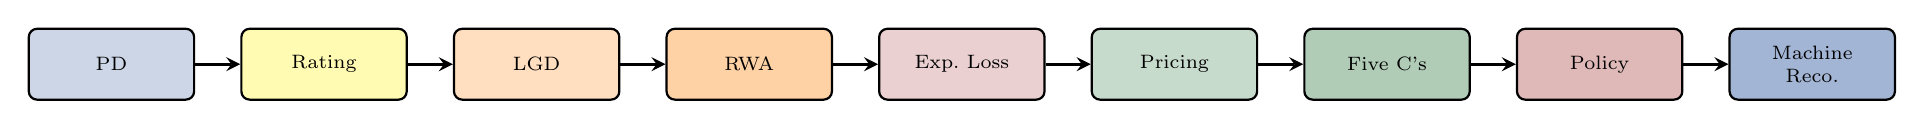
\begin{tikzpicture}[
    sbox/.style={draw, rounded corners=3pt, align=center, minimum width=2.1cm, minimum height=0.9cm,
                 inner sep=3pt, font=\scriptsize, thick},
    arr/.style={->, very thick, >=stealth}
]
\node[sbox, fill=steelblue!25]   (pd)  at (0,0)  {PD};
\node[sbox, fill=yellow!30]      (rat) at (2.7,0) {Rating};
\node[sbox, fill=orange!25]      (lgd) at (5.4,0) {LGD};
\node[sbox, fill=orange!35]      (rwa) at (8.1,0) {RWA};
\node[sbox, fill=darkred!20]     (el)  at (10.8,0) {Exp.\ Loss};
\node[sbox, fill=forestgreen!25] (prc) at (13.5,0) {Pricing};
\node[sbox, fill=forestgreen!35] (fc)  at (16.2,0) {Five C's};
\node[sbox, fill=darkred!30]     (pol) at (18.9,0) {Policy};
\node[sbox, fill=steelblue!45]   (rec) at (21.6,0) {Machine\\Reco.};
\draw[arr] (pd) -- (rat); \draw[arr] (rat) -- (lgd); \draw[arr] (lgd) -- (rwa);
\draw[arr] (rwa) -- (el); \draw[arr] (el) -- (prc); \draw[arr] (prc) -- (fc);
\draw[arr] (fc) -- (pol); \draw[arr] (pol) -- (rec);
\end{tikzpicture}%
}
\end{center}
\vspace{6pt}
\begin{columns}[T]
  \column{0.48\textwidth}
    \footnotesize\textbf{How it's explained, not just scored}
    \begin{itemize}\setlength\itemsep{3pt}\footnotesize
      \item[\small$\bullet$] SHAP attribution --- top factors pushing PD up/down, in plain language
      \item[\small$\bullet$] Peer comparison --- segment-scoped benchmark against approved
            borrowers in the same exposure class
      \item[\small$\bullet$] Counterfactual recourse --- ``what would need to change to qualify''
            for borderline/declined applicants
    \end{itemize}
  \column{0.48\textwidth}
    \footnotesize\textbf{How it's presented --- two views, one finding}
    \begin{itemize}\setlength\itemsep{3pt}\footnotesize
      \item[\small$\bullet$] \textbf{Underwriter report} (internal, 6 sections): Risk Assessment,
            Five C's, Peer Comparison, Improvement Pathways, AIRB Regulatory Detail, Credit Decision
      \item[\small$\bullet$] \textbf{Applicant letter} (adverse-action style) --- decision and
            reason, not the technical internals
    \end{itemize}
\end{columns}
\vspace{6pt}
\begin{alertblock}{Output object}
  \footnotesize
  The \textbf{Machine Recommendation (M)} bundles the risk estimate, policy result,
  confidence/sensitivity, and required-control-level routing into one hash-stamped record ---
  this is what the RM reviews next.
\end{alertblock}
\end{frame}

% SLIDE — ROLE OF THE RM
\begin{frame}{Role of the Relationship Manager}
\vspace{-2pt}
\begin{block}{Where the RM sits}
  \footnotesize
  The Human (H) node between the \textbf{Machine Recommendation (M)} and the
  \textbf{Org Decision (O)} --- the RM does not replace the model, and the model does not
  replace the RM.
\end{block}
\vspace{6pt}
\begin{columns}[T]
  \column{0.5\textwidth}
    \footnotesize\textbf{What the RM actually does}
    \begin{itemize}\setlength\itemsep{3pt}\footnotesize
      \item[\small$\bullet$] Reviews the Machine Recommendation --- SHAP factors, peer comparison,
            counterfactual recourse, policy flags
      \item[\small$\bullet$] \textbf{Two actions only} --- Accept or Reject, each requiring a
            $\geq$20-character rationale; both finalise immediately, no partial states
      \item[\small$\bullet$] Whether the RM can decide \emph{alone} depends on the DoA control
            level already computed (\texttt{RM\_SINGLE} / \texttt{FOUR\_EYES} / \texttt{COMMITTEE}
            / \texttt{AUTO\_DECLINE}) --- the platform tells the RM up front whether this case is
            even theirs to close
      \item[\small$\bullet$] After a decision, the RM can trigger PDF report generation; every
            action is hash-chained into the case's audit trail
    \end{itemize}
  \column{0.46\textwidth}
    \begin{alertblock}{What the RM does \emph{not} do}
      \footnotesize
      \begin{itemize}\setlength\itemsep{3pt}
        \item[\small$\bullet$] Re-enter borrower data
        \item[\small$\bullet$] Override the model's PD
        \item[\small$\bullet$] Approve outside their delegated authority
      \end{itemize}
      \vspace{3pt}
      These are \textbf{structurally prevented}, not just discouraged by policy.
    \end{alertblock}
\end{columns}
\end{frame}

% ===========================================================
% Further content slides go here — added incrementally on request.
% ===========================================================

\end{document}
